
%(BEGIN_QUESTION)
% Copyright 2012, Tony R. Kuphaldt, released under the Creative Commons Attribution License (v 1.0)
% This means you may do almost anything with this work of mine, so long as you give me proper credit

An H1 Fieldbus segment which had been working just fine for years suddenly failed, and is now being diagnosed by an instrument technician.  The technician has connected a multimeter to the network wiring as shown, and obtains a reading of 0.000 volts AC:

$$\includegraphics[width=15.5cm]{i02138x01.eps}$$

Identify {\it two} different faults that could account for the non-function of the Fieldbus network, based also on the multimeter indication shown here.

\vskip 30pt

\underbar{file i02138}
%(END_QUESTION)





%(BEGIN_ANSWER)

\begin{itemize}
\item{} LAS device has failed, with no backup LAS in the system
\item{} Open wire between TB43-24 and TB105-1
\item{} Open wire between TB43-25 and TB105-2
\item{} Shorted trunk cable (two power/signal conductors shorted together)
\item{} 24 VDC power supply dead
\end{itemize}

\vskip 10pt

It should be noted that a ground fault would not account for 0 volts AC registered by the multimeter, and neither would any problem with the cable shield.

%(END_ANSWER)





%(BEGIN_NOTES)

{\bf This question is intended for exams only and not worksheets!}

%(END_NOTES)


